\documentclass{article}

\usepackage[utf8]{inputenc}
\usepackage[T1]{fontenc}
\usepackage{lipsum}
\usepackage{graphicx}
\usepackage{amsmath}
\usepackage[margin=1in]{geometry}
\usepackage{titlesec}
\usepackage{enumitem}

\titleformat{\section}
{\LARGE\bfseries}{\thesection}{1em}{}

\titleformat{\subsection}
{\Large\bfseries}{\thesection}{1em}{}

\begin{document}
\pagestyle{empty}
\section*{Modern Patterns}
\large

\subsection*{Introduzione}
\large
Obiettivi:
\begin{itemize}
    \renewcommand{\labelitemi}{-}
    \itemsep0em
    \item Comprendere come attuare propriamente pattern moderni.
\end{itemize}

\subsection*{Null Object (Modern Pattern)}
\large
\textit{Problema}\\
Come evitare che venga restituito un valore "null" quando viene richiesto un riferimento ad un'interfaccia?\vspace*{14pt}\\
\textit{Soluzione}\\
Si utilizza un oggetto che implementa l’interfaccia attesa, ma in cui il corpo del metodo è vuoto\vspace*{14pt}\\
\textit{Null Object} permette di semplificare l'utilizzo delle dipendenze che possono essere indefinite. Ciò si ottiene utilizzando istanze di una classe concreta che implementa un'interfaccia nota, invece di riferimenti null. In primo luogo, viene realizzata una classe astratta contenente diverse operazioni da eseguire, classi concrete che estendono questa classe e infine una classe di oggetti null che fornisce un'implementazione \textit{do-nothing}, la quale verrà utilizzata senza problemi dove potrebbe essere riscontrato il valore null.\vspace*{14pt}\\
\textit{Caso di studio}\\
\begin{center}
    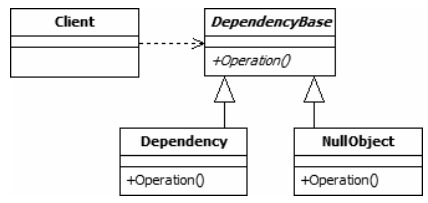
\includegraphics[width=0.45\textwidth]{foto 1.png}
\end{center}
Si analizzano le entità che rappresentano la raffigurazione, in cui:
\begin{itemize}[label={-}]
    \itemsep0em
    \item \textit{Client}, ha una dipendenza che può essere richiesta o meno. Laddove non sia richiesta alcuna funzionalità nella dipendenza, eseguirà i metodi di un oggetto null
    \item \textit{DependencyBase}, superclasse per le varie dipendenze disponibili che il Client può utilizzare. Laddove la superclasse non fornisce funzionalità condivise, può essere sostituita con un'interfaccia
    \item \textit{Dependency}, dipendenza funzionale che può essere utilizzata dal Client
    \item \textit{NullObject}, può essere utilizzata come dipendenza dal Client. Non contiene funzionalità ma implementa tutti i membri definiti dalla classe astratta \textit{DependencyBase}.
\end{itemize}
Concludendo, il design pattern Null Object risulta funzionare nell'evitare problematiche relative all'eccezione \textit{NullPointerException}, al tempo stesso però non sarà possibile controllare la consistenza di un oggetto.

\subsection*{Dipendency Injection (Modern Pattern)}
\large
\textit{Problema}\\
Come creare un'istanza di un'entità software senza che sia specificata la classe?\vspace*{14pt}\\
Tipicamente tale problematica avviene qualora classi di alto livello richiedano comportamenti sviluppati in classi di basso livello. Rispetto a capitoli precedenti, sono stati introdotti approcci capaci di rispondere attivamente alla domanda, come la \textit{sovvrapposizione} di layer \textit{astratti} tra le due entità, affinchè risultino totalmente isolate, oppure attraverso l'impiego di \textit{pattern creazionali}, come \textit{Factory Method}, in cui è delegata la responsabilità a termini software dediti solamente alla concretizzazione di istanze che saranno successivamente restituite al richiedente; tuttavia esiste un meccanismo migliorativo in grado di eliminare qualsiasi incertezza relativa ad errate gestioni di dipendenze, definita \textbf{Dipendency Injection}.\vspace*{14pt}\\
\textit{Soluzione}\\
Dipendency Injection crea un grafo di dipendenze che adotti l'inversione di controllo per individuare gli oggetti associati, in maniera tale che le dipendenze siano immesse dal nucleo verso i nodi esterni.\vspace*{14pt}\\
Il \textit{pattern} descritto è in grado di stabilire concretamente la rottura delle dipendenze tra \textit{LLC} e \textit{HLC}, contrariamente alle soluzioni precedenti, ossia mediante l'implementazione della sintassi \textit{new(...)} oppure tramite \textit{factories}, attuando la delega comportamentale.\vspace*{14pt}\\
\end{document}